%%----------------------------------------------------------------------------
%% Onderzoekstechnieken: Analyse van 2 kwantitatieve variabelen
%%----------------------------------------------------------------------------

\documentclass[aspectratio=169]{beamer}

%==============================================================================
% Aanloop
%==============================================================================

%---------- Vormgeving --------------------------------------------------------

\usetheme{hogent}

\usecolortheme{hgwhite} % witte achtergrond, zwarte tekst

\usepackage{graphicx,multicol}
\usepackage{comment,enumerate,hyperref}
\usepackage{amsmath,amsfonts,amssymb}
\usepackage[dutch]{babel}
\usepackage{multirow}
\usepackage{eurosym}
\usepackage{listings}
\usepackage{textcomp}
\usepackage{framed}
\usepackage{wrapfig}
\usepackage{tabu} %needed for \tabulinesep
\usepackage{wrapfig}
\usepackage{pgf-pie}
\usepackage{pgfplots}
\usepackage{booktabs}
\usepackage{pgfplotstable}
\usepackage{changepage}
\usepackage{ulem} % for \sout{text} (strikethrough)
\usepackage{fancyvrb} % for \begin{Verbatim} (LaTeX controls within verbatim)

%---------- Configuratie ------------------------------------------------------

\pgfplotsset{compat=1.16}
\usetikzlibrary{arrows,shapes,backgrounds,positioning,shadows}
\usetikzlibrary{pgfplots.statistics}

%---------- Commando-definities -----------------------------------------------

\newcommand{\tabitem}{~~\llap{\textbullet}~~}
\newcommand{\alertbox}[2][hgblue]{%
  \setbeamercolor{alertbox}{bg=#1,fg=white}
  \begin{beamercolorbox}[sep=2pt,center]{alertbox}
    \textbf{#2}
  \end{beamercolorbox}
}
\pgfmathdeclarefunction{gauss}{2}{%
  \pgfmathparse{1/(#2*sqrt(2*pi))*exp(-((x-#1)^2)/(2*#2^2))}%
}

%---------- Info over de presentatie ------------------------------------------

\title{Hst 6. Analyse van 2 kwantitatieve variabelen}
\subtitle{Onderzoekstechnieken}
\author{Jens Buysse \and Wim {De Bruyn} \and Pieter-Jan Maenhout \and Bert {Van Vreckem}}
\date{AJ 2019-2020}

%==============================================================================
% Inhoud presentatie
%==============================================================================

\begin{document}

\begin{frame}
  \maketitle
\end{frame}

\begin{frame}
  \frametitle{What's on the menu today?}
  
  \tableofcontents
\end{frame}

\begin{frame}
  \frametitle{Leerdoelen}
  
  \begin{itemize}
    \item Regressie-analyse
    \item Covariantie, correlatiecoëfficiënt, determinatiecoëfficiënt
  \end{itemize}
\end{frame}

\begin{frame}
  \frametitle{Overzicht}
    \centering
    \begin{tabular}{lll}
    	\toprule
    	\textbf{Onafhankelijke} & \textbf{Afhankelijke} & \textbf{Toets/metriek}        \\
    	\midrule
    	Kwalitatief             & Kwalitatief           & $\chi^2$-toets                \\
    	                        &                       & Cramér's $V$                  \\
    	Kwalitatief             & Kwantitatief          & $t$-toets voor 2 steekproeven \\
    	                        &                       & Cohen's $d$                   \\
    	Kwantitatief            & Kwantitatief          & ---                           \\
    	                        &                       & Regressie, correlatie         \\
    	\bottomrule
    \end{tabular}
\end{frame}

\section{Lineaire Regressie}

\begin{frame}
  \frametitle{Lineaire regressie}
  \alertbox{Bij \textcolor{hgyellow}{regressie} gaan we proberen een \textcolor{hgyellow}{consistente} en \textcolor{hgyellow}{systematische} koppeling tussen de variabelen te vinden.}
  
  
  \begin{enumerate}
    \item \textbf{Monotoon:} algemene richting van de samenhang tussen de twee variabelen kan aangeduid worden (stijgend/dalend).
    \item \textbf{Niet-monotoon:}  aanwezigheid (of afwezigheid) van de ene variabele systematisch gerelateerd aan de aanwezigheid (of afwezigheid) van een andere variabele.
  \end{enumerate}
\end{frame}

\begin{frame}
  \frametitle{Lineaire regressie}
  Lineair verband: een rechtlijnige samenhang tussen een onafhankelijke en afhankelijke variabele, waarbij kennis van de onafhankelijke variabele kennis over de afhankelijke variabele geeft.
  \begin{itemize}
    \item Aanwezigheid
    \item Richting: dalend of stijgend?
    \item Sterke van het verband: sterk, gematigd, niet bestaand \dots
  \end{itemize}
\end{frame}

\begin{frame}
  \frametitle{Lineaire regressie}
  \centering
  \begin{tikzpicture}
  \begin{axis}[
  axis x line=middle,
  axis y line=middle,
  enlarge y limits=true,
  width=.9\textwidth, height=.9\textheight,     % size of the image
  grid = major,
  grid style={dashed, gray!30},
  ylabel=$y$,
  xlabel=$x$,
  legend style={at={(0.1,-0.1)}, anchor=north}
  ]
  \addplot[only marks] table  {data/regressie.dat};
  %\addplot [no markers, thick, red] table [y={create col/linear regression={y=y}}] {data/regressie.dat};
  \end{axis}
  \end{tikzpicture}
\end{frame}

\begin{frame}
  \frametitle{Lineaire regressie}
  \centering
  \begin{tikzpicture}
  \begin{axis}[
  axis x line=middle,
  axis y line=middle,
  enlarge y limits=true,
  width=.9\textwidth, height=.9\textheight,     % size of the image
  grid = major,
  grid style={dashed, gray!30},
  ylabel=$y$,
  xlabel=$x$,
  legend style={at={(0.1,-0.1)}, anchor=north}
  ]
  \addplot[only marks] table  {data/regressie.dat};
  \addplot [no markers, thick, red] table [y={create col/linear regression={y=y}}] {data/regressie.dat};
  \end{axis}
  \end{tikzpicture}
\end{frame}

\begin{frame}[plain]
  \frametitle{Kleinste kwadratenmethode}
  \framesubtitle{Voorbeeld}
  \begin{columns}
    \begin{column}{0.5\textwidth}
      
      \begin{figure}
        \centering
        
\includegraphics[height=.6\textheight]{les3-santa.png}
        \label{fig:les3-santa}
      \end{figure}
      
    \end{column}
    \begin{column}{0.5\textwidth}
      
      \begin{figure}
        \centering
        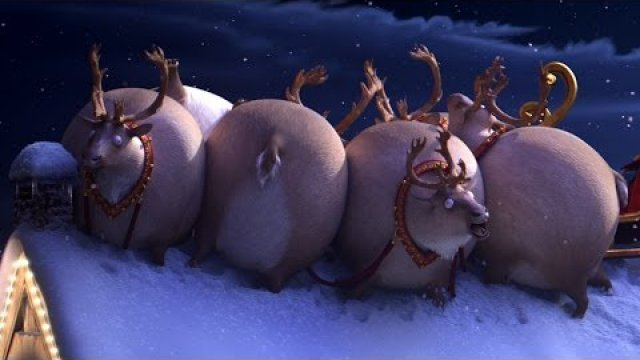
\includegraphics[width=1.00\textwidth]{les3-reindeer.jpg}
        \label{fig:les3-reindeer}
      \end{figure}
      
    \end{column}
  \end{columns}

  \bigskip
  De Kerstman wil zijn rendieren vetmesten. Is er een verband
  tussen de hoeveelheid eiwitten in het dieet van de rendieren
  en hun gewichtstoename?
  
\end{frame}

\begin{frame}
  \frametitle{Kleinste kwadratenmethode}
  \framesubtitle{Voorbeeld}
  
  \begin{table}[h]
    \centering
    \small
    \begin{tabular}{@{}rr@{}} \toprule
      Eiwitgehalte\%& Gewichtstoename (gram)  \\
      \midrule
      0   & 177 \\
      10  & 231 \\
      20  & 249 \\
      30  & 348 \\
      40  & 361 \\
      50  & 384 \\
      60  & 404 \\
      \bottomrule
    \end{tabular}
  \end{table}
\end{frame}

\begin{frame}
  \frametitle{Kleinste kwadratenmethode}
  \framesubtitle{Voorbeeld}
  
  \centering
  \begin{tikzpicture}
  \begin{axis}[
  axis x line=middle,
  axis y line=middle,
  enlarge y limits=true,
  width=.9\textwidth, height=.9\textheight,     % size of the image
  grid = major,
  grid style={dashed, gray!30},
  ylabel=gewichtstoename (g),
  xlabel=eiwitgehalte (\%),
  legend style={at={(0.1,-0.1)}, anchor=north}
  ]
  \addplot[only marks] table  {data/santa.txt};
  % \addplot [no markers, thick, red] table [y={create col/linear regression={y=y}}] {data/santa.txt};
  \end{axis}
  \end{tikzpicture}
\end{frame}

\begin{frame}
  \frametitle{Kleinste kwadratenmethode}
  \framesubtitle{Voorbeeld}
  
  \begin{table}[h] \centering \footnotesize
    \begin{tabular}{@{}llllll@{}}
      \toprule
      $x$   & $y$     & $x-\overline{x}$    & $y - \overline{y}$        & $(x-\overline{x})(y - \overline{y})$       &  $(x-\overline{x})^{2}$    \\ \midrule
      0  & 177 & -30 & -130,71 & 3921,3 & 900  \\
      10 & 231 & -20 & -76,71  & 1534,2 & 400  \\
      20 & 249 & -10 & -58,71  & 587,1  & 100  \\
      30 & 348 & 0   & 40,29   & 0      & 0    \\
      40 & 361 & 10  & 53,29   & 532,9  & 100  \\
      50 & 384 & 20  & 76,29   & 1525,8 & 400  \\
      60 & 404 & 30  & 96,29   & 2888,7 & 900  \\
      &     &     &         & 10990  & 2800 \\ \bottomrule
    \end{tabular}
    \caption{Berekeningen die nodig zijn voor het toepassen van de kleinste kwadratenmethode.}
    \label{tab:rendieren2}
  \end{table}
\end{frame}

\begin{frame}
  \frametitle{Kleinste kwadratenmethode}
  \framesubtitle{Formule}
  
  De regressierechte heeft als vergelijking:
  
  \[ \hat{y} = \beta_1 x + \beta_0 \]
  
  met:
  
  \[ \beta_{1} = \frac{\sum_{i=1}^{n} (x_{i}-\overline{x})(y_{i} - \overline{y})}{\sum_{i=1}^{n} (x-\overline{x})^{2}} = \frac{10990}{2800} = 3.925 \]
  \[ \beta_{0} = \overline{y} - \beta_{1} \overline{x} = 307.7143 - 3.925 \times 30 = 189.96 \]
  
  Opm: $\hat{y}$ betekent ``een schatting voor $y$''
\end{frame}

\begin{frame}
  \frametitle{Kleinste kwadratenmethode}
  \framesubtitle{Voorbeeld}
  
  \centering
  \begin{tikzpicture}
  \begin{axis}[
  axis x line=middle,
  axis y line=middle,
  enlarge y limits=true,
  width=.9\textwidth, height=.9\textheight,     % size of the image
  grid = major,
  grid style={dashed, gray!30},
  ylabel=gewichtstoename (g),
  xlabel=eiwitgehalte (\%),
  legend style={at={(0.1,-0.1)}, anchor=north}
  ]
  \addplot[only marks] table  {data/santa.txt};
  \addplot [no markers, thick, red] table [y={create col/linear regression={y=y}}] {data/santa.txt};
  \end{axis}
  \end{tikzpicture}
\end{frame}

\section{Correlatieco\"effici\"ent en determinatieco\"effci\"ent}

\begin{frame}
  \frametitle{Covariantie}
  
  \alertbox{Covariantie is een maat die aangeeft of een verband tussen twee variabelen stijgend dan wel dalend is.}
  
  \[ \mathrm{Cov}(X, Y) = \frac{1}{n} \sum_{i = 1}^{n} (x_i - \overline{x}) (y_i - \overline{y}) \]
  
  $\mathrm{Cov} > 0$: stijgend
  
  $\mathrm{Cov} \approx 0$: geen verband
  
  $\mathrm{Cov} < 0$: dalend
\end{frame}

\begin{frame}
  \frametitle{Covariantie}
  We plotten de gezinsgrootte van 15 families tot de gezinsgrootte van de moeder toen ze klein was.
  
  \centering
  \begin{tikzpicture}
  \begin{axis}[
  axis x line=middle,
  axis y line=middle,
  enlarge y limits=true,
  width=.9\textwidth, height=.9\textheight,     % size of the image
  grid = major,
  grid style={dashed, gray!30},
  ylabel=gezinsgrootte moeder,
  xlabel=gezinsgrootte,
  legend style={at={(0.1,-0.1)}, anchor=north}
  ]
  \addplot[only marks] table  {data/families.txt};
  \addplot [no markers, thick, red] table [y={create col/linear regression={y=y}}] {data/families.txt};
  \end{axis}
  \end{tikzpicture}
  We vinden $\overline{x} = 3$ en $\overline{y} = 4.3$.
\end{frame}

\tikzset{small dot/.style={fill=black, circle,scale=0.2}}
\tikzset{every pin/.style={draw=black,fill=yellow!10}}

\begin{frame}
  \frametitle{Covariantie bij lineair verband}
  \centering
  \begin{tikzpicture}
  \begin{axis}[
  axis x line=middle,
  axis y line=middle,
  enlarge y limits=true,
  width=.9\textwidth, height=.9\textheight,     % size of the image
  grid = major,
  grid style={dashed, gray!30},
  ylabel=gezinsgrootte moeder,
  xlabel=gezinsgrootte,
  legend style={at={(0.1,-0.1)}, anchor=north}
  ]
  \draw (axis cs:3,0)--(axis cs:3,8);
  \draw (axis cs:0,4.3)--(axis cs:6,4.3);
  \node[small dot, pin=120:{$III$}] at (axis cs:1.9,6) {};
  \node[small dot, pin=120:{$I$}] at (axis cs:4.5,6) {};
  \node[small dot, pin=120:{$II$}] at (axis cs:1.9,2) {};
  \node[small dot, pin=120:{$IV$}] at (axis cs:4.5,2) {};
  \addplot[only marks] table  {data/families.txt};
  \end{axis}
  \end{tikzpicture}
\end{frame}

\begin{frame}
  \frametitle{Covariantie bij willekeurigheid}
  \centering
  \begin{tikzpicture}
  \begin{axis}[
  axis x line=middle,
  axis y line=middle,
  enlarge y limits=true,
  width=.9\textwidth, height=.9\textheight,     % size of the image
  grid = major,
  grid style={dashed, gray!30},
  ylabel=gezinsgrootte moeder,
  xlabel=geboortedatum moeder,
  legend style={at={(0.1,-0.1)}, anchor=north}
  ]
  \draw (axis cs:1942.625,0)--(axis cs:1942.625,6);
  \draw (axis cs:1930,3.4375)--(axis cs:1955,3.4375);
  \node[small dot, pin=120:{$III$}] at (axis cs:1935,5) {};
  \node[small dot, pin=120:{$I$}] at (axis cs:1950,5) {};
  \node[small dot, pin=120:{$II$}] at (axis cs:1935,2) {};
  \node[small dot, pin=120:{$IV$}] at (axis cs:1950,2) {};
  \addplot[only marks] table  {data/families2.txt};
  \end{axis}
  \end{tikzpicture}
  We vinden $\overline{x} = 1942.625$ en $\overline{y} = 3.4375$.
\end{frame}

\begin{frame}
  \frametitle{Pearson correlatiecoëfficiënt}
  
  \alertbox{De \textcolor{hgyellow}{Pearson correlatiecoëfficiënt} $R$ is een maat voor de sterkte van de lineaire samenhang tussen $x$ en $y$}
  
  \begin{align}
  R & = \frac{Cov(X, Y)}{\sigma_{x} \sigma_{y}} \\
  & = \frac{\sum_{i = 1}^{n} (x_i - \overline{x}) (y_i - \overline{y})}
  {\sqrt{\sum_{i = 1}^n (x_i - \overline{x})^2}
    \sqrt{\sum_{i = 1}^n (y_i - \overline{y})^2}}
  \end{align}
  
  \[ R \in [-1, +1] \]
  
\end{frame}


\begin{frame}
  \frametitle{Interpretatie correlateco\"effici\"ent}
  
  \centering
  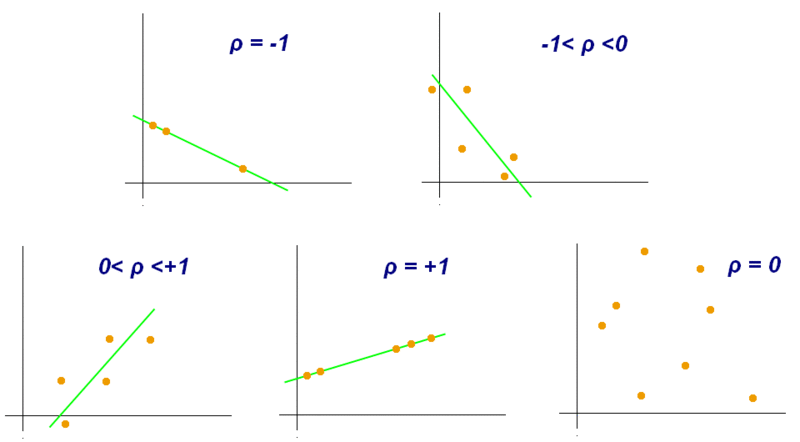
\includegraphics[height=.8\textheight]{les3-regressie.png}
  
\end{frame}

\begin{frame}
  \frametitle{Determinatiecoëfficiënt}
  \alertbox{De \textcolor{hgyellow}{determinatiecoëfficiënt} $R^2$ verklaart het percentage van de variantie van de waargenomen waarden t.o.v. de regressierechte.}
  
  $R^2$: percentage variantie in waarnemingen verklaard door de regressierechte
  
  $1 - R^2$: percentage variantie waarnemingen \textit{niet} verklaard door de regressie
  
\end{frame}

\begin{frame}[plain]
  \frametitle{Determinatieco\"effici\"ent}
  \begin{figure}
    \resizebox{.7\textwidth}{.7\textheight}{
      \begin{tikzpicture}
        \begin{axis}[
        axis x line=middle,
        axis y line=middle,
        enlarge y limits=true,
        width=.9\textwidth, height=.9\textheight,     % size of the image
        grid = major,
        grid style={dashed, gray!30},
        ylabel=gewichtstoename (g),
        xlabel=eiwitgehalte (\%),
        legend style={at={(0.1,-0.1)}, anchor=north}
        ]
        \addplot[only marks] table  {data/santa.txt};
        \addplot [no markers, thick, red] table [y={create col/linear regression={y=y}}] {data/santa.txt};
        \addplot [mark=none, color=red] coordinates {
          (0,177) (0,189.9643)
        };
        \addplot [mark=none, color=red] coordinates {
          (10,231) (10,229.2143)
        };
        \addplot [mark=none, color=red] coordinates {
          (20,249) (20,268.4643)
        };
        \addplot [mark=none, color=red] coordinates {
          (30,348) (30,307.7143)
        };
        \addplot [mark=none, color=red] coordinates {
          (40,361) (40,346.9643)
        };
        \addplot [mark=none, color=red] coordinates {
          (50,384) (50,386.2143)
        };
        \addplot [mark=none, color=red] coordinates {
          (60,404) (60,425.4643)
        };
        
        \end{axis}
      \end{tikzpicture}
    }
    \label{fig:rendierenFiguur2}
    \caption{Deviaties tot de regressierechte: aanname $x$ geeft extra informatie voor het voorspellen van $y$.}
  \end{figure}
\end{frame}

\begin{frame}[plain]
  \begin{figure}
    \resizebox{.7\textwidth}{.7\textheight}{
      \begin{tikzpicture}
        \begin{axis}[
        axis x line=middle,
        axis y line=middle,
        enlarge y limits=true,
        width=.9\textwidth, height=.9\textheight,     % size of the image
        grid = major,
        grid style={dashed, gray!30},
        ylabel=gewichtstoename (g),
        xlabel=eiwitgehalte (\%),
        ]
        \addplot[only marks] table  {data/santa.txt};
        \addplot [mark=none, color=black] coordinates {
          (0,307.71) (60,307.71)
        };
        \addplot [mark=none, color=red] coordinates {
          (0,177) (0,307.71)
        };
        \addplot [mark=none, color=red] coordinates {
          (10,231) (10,307.71)
        };
        \addplot [mark=none, color=red] coordinates {
          (20,249) (20,307.71)
        };
        \addplot [mark=none, color=red] coordinates {
          (30,348) (30,307.71)
        };
        \addplot [mark=none, color=red] coordinates {
          (40,361) (40,307.71)
        };
        \addplot [mark=none, color=red] coordinates {
          (50,384) (50,307.71)
        };
        \addplot [mark=none, color=red] coordinates {
          (60,404) (60,307.71)
        };
        
        \end{axis}
      \end{tikzpicture}
    }
    \label{fig:rendierenFiguur3}
    \caption{Deviaties tot de gemiddelde van y: aanname $x$ geeft geen informatie voor het voorspellen van $y$ ($\overline{y} =307.71$).}
  \end{figure}
\end{frame}

\begin{frame}
  \frametitle{Correlatieco\"effici\"ent en determinatieco\"effci\"ent}
  \centering
  \begin{table} \small
    \begin{tabular}{@{}rrrr@{}} \toprule
      $|R|$ & $R^{2}$ & Verklaarde variantie &  Interpretatie \\
      \midrule
      $< 0,3$       & $< 0,1$       & $< 10\%$    & zeer zwak \\
      $0,3 - 0,5$   & $0,1 - 0,25$ & $10 - 25\%$ & zwak \\
      $0,5 - 0,7$   & $0,25 - 0,5$  & $25 - 50\%$ & matig\\
      $0,7 - 0,85$  & $0,5 - 0,75$  & $50 - 75\%$ & sterk\\
      $0,85 - 0,95$ & $0,75 - 0,9$  & $75 - 90\%$ & zeer sterk\\
      $> 0,95$      & $> 0,9$       & $>90\%$     & uitzonderlijk(!)\\
      \bottomrule
    \end{tabular}
  \end{table}
  
\end{frame}

\begin{frame}
  \frametitle{Sterkte verband rendieren}
  \begin{columns}
    \begin{column}{0.5\textwidth}
      \begin{table}[h] \centering \small
        \begin{tabular}{@{}rrr@{}} \toprule
          $(x-\overline{x})$ & $(y - \overline{y})$ & $(x-\overline{x})(y - \overline{y})$ \\
          \midrule
          $-30$ & $-130.714$ & $3921.429$ \\
          $-20$ & $-76.7143$ & $1534.286$ \\
          $-10$ & $-58.7143$ & $587.1429$\\
          $0$   & $40.28571$ & $0$\\
          $10$  & $53.28571$ & $532.8571$\\
          $20$  & $76.28571$ & $1525.714$\\
          $30$  & $96.28571$ & $2888.571$\\
          \bottomrule
        \end{tabular}
      \end{table}
    \end{column}
    \begin{column}{0.5\textwidth}
      \[ \sum_{i}^{n} (x-\overline{x})(y - \overline{y}) = 10990 \]
      \[ Cov = \frac{10990}{7} = 1570 \]
      \[ \sigma_{x} = 20 \]
      \[ \sigma_{y} = 81.03 \]
      \[ R = \frac{1570}{20 \times 81.03} = 0.96 \]
      \[ R^{2} = 0.93 \]
    \end{column}
  \end{columns}
\end{frame}

\begin{frame}
  \frametitle{Overwegingen}
  \begin{itemize}
    \item Bij de correlatiecoëfficiënt wordt er alleen naar het verband tussen twee variabelen gekeken. Er wordt niet gekeken naar interacties met andere variabelen.
    \item Er wordt bij de correlatiecoëfficiënt expliciet niet uitgegaan van een oorzaak-en gevolg verband
    \item De product-momentcorrelatiecoëfficiënt van Pearson drukt slechts lineaire verbanden uit
  \end{itemize}
\end{frame}

\end{document}